% inspired from http://tex.stackexchange.com/questions/47469/how-do-i-make-an-unbalanced-binary-tree
\documentclass{article}

\usepackage{tikz}
\usepackage{tikz-qtree}
\usetikzlibrary{trees}
\usetikzlibrary{shapes, positioning, arrows, calc}

\begin{document}

% Intro : représentation des sous problèmes
         
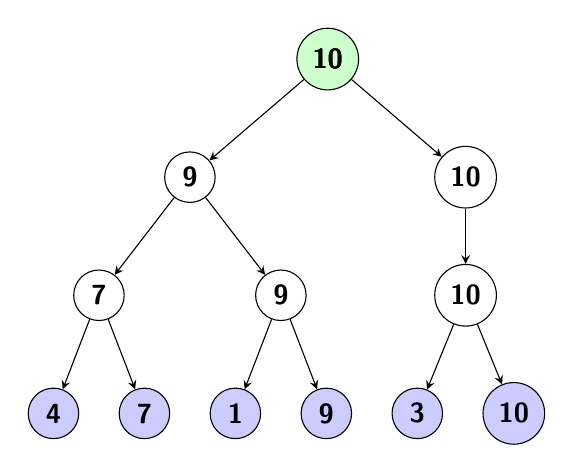
\begin{tikzpicture}[every tree node/.style = {minimum width = 0.5cm, draw, circle},
style = {->, >=stealth},
edge from parent/.style = {draw, edge from parent path = {(\tikzparentnode) -- (\tikzchildnode)}},
level distance = 1.5cm, sibling distance = 0.5cm,
font = \sffamily\bfseries,
every leaf node/.style = {fill = blue!20}]
\node[fill = green!20, circle] {10};
\Tree
[.10
	[.9
		[.7 4 7 ]
		[.9 1 9 ]
	]
	[.10 
		[.10 3 10 ]
	]
]
\end{tikzpicture}

% Exemple arbre binaire

\vspace{2cm}

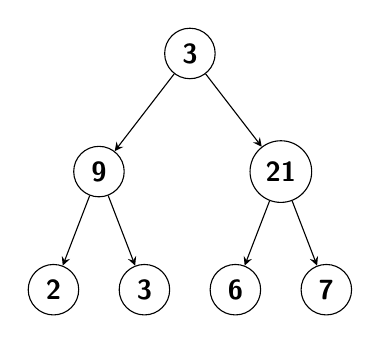
\begin{tikzpicture}[every tree node/.style = {minimum width = 0.5cm, draw, circle},
style = {->, >=stealth},
edge from parent/.style = {draw, edge from parent path = {(\tikzparentnode) -- (\tikzchildnode)}},
level distance = 1.5cm, sibling distance = 0.5cm,
font = \sffamily\bfseries]
\Tree
[.3
	[.9 2 3 ]
	[.21 6 7 ]
]
\end{tikzpicture}

% Implémentation d'un arbre binaire dans un tableau

\vspace{2cm}

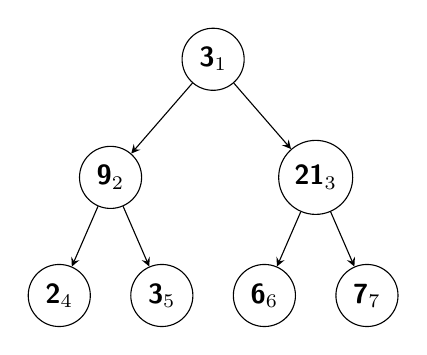
\begin{tikzpicture}[every tree node/.style = {minimum width = 0.5cm, draw, circle},
style = {->, >=stealth},
edge from parent/.style = {draw, edge from parent path = {(\tikzparentnode) -- (\tikzchildnode)}},
level distance = 1.5cm, sibling distance = 0.5cm,
font = \sffamily\bfseries]
\Tree
[.3$_1$
	[.9$_2$ 2$_4$ 3$_5$ ]
	[.21$_3$ 6$_6$ 7$_7$ ]
]
\end{tikzpicture}

\vspace{0.5cm}

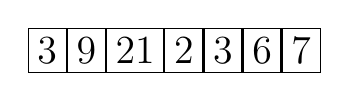
\begin{tikzpicture}
\node [font=\sffamily\Large\bfseries, draw, anchor=center] (first) {$3$};
\node [font=\sffamily\Large\bfseries, draw, anchor=center, right=0cm of first] (second) {$9$};
\node [font=\sffamily\Large\bfseries, draw, anchor=center, right=0cm of second] (third) {$21$};
\node [font=\sffamily\Large\bfseries, draw, anchor=center, right=0cm of third] (fourth) {$2$};
\node [font=\sffamily\Large\bfseries, draw, anchor=center, right=0cm of fourth] (fifth) {$3$};
\node [font=\sffamily\Large\bfseries, draw, anchor=center, right=0cm of fifth] (sixth) {$6$};
\node [font=\sffamily\Large\bfseries, draw, anchor=center, right=0cm of sixth] (seventh) {$7$};
\end{tikzpicture}

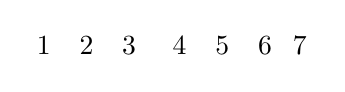
\begin{tikzpicture}
\node [font=\sffamily\Large\bfseries, anchor=center] (first) {$_1$};
\node [font=\sffamily\Large\bfseries, anchor=center, right=0.1cm of first] (second) {$_2$};
\node [font=\sffamily\Large\bfseries, anchor=center, right=0.1cm of second] (third) {$_3$};
\node [font=\sffamily\Large\bfseries, anchor=center, right=0.2cm of third] (fourth) {$_4$};
\node [font=\sffamily\Large\bfseries, anchor=center, right=0.1cm of fourth] (fifth) {$_5$};
\node [font=\sffamily\Large\bfseries, anchor=center, right=0.1cm of fifth] (sixth) {$_6$};
\node [font=\sffamily\Large\bfseries, anchor=center, right=0cm of sixth] (seventh) {$_7$};
\end{tikzpicture}

\end{document}